\documentclass{standalone}
\usepackage{tikz}
\usetikzlibrary{patterns, positioning}

\begin{document}
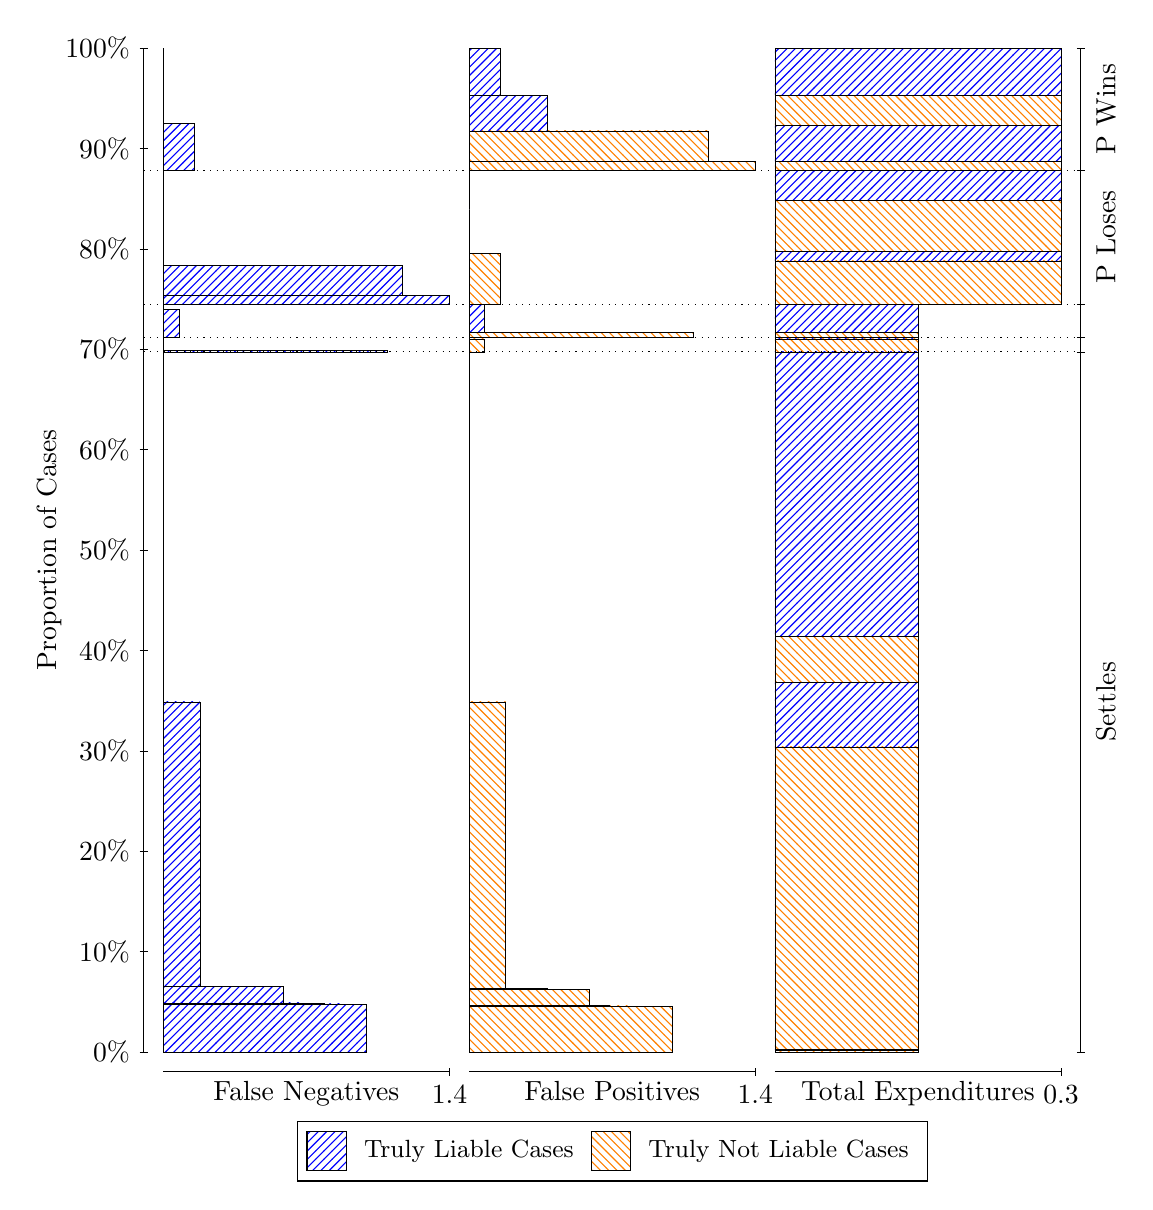
\begin{tikzpicture}
\draw[black, very thin] (1.5,1.75) -- (1.5,14.5);
\node[rotate=90, anchor=center] at (0.3, 8.125) {Proportion of Cases};
\draw[black, very thin] (1.45,1.75) -- (1.55,1.75);
\node[anchor=east] at (1.45, 1.75) {0\%};
\draw[black, very thin] (1.45,3.025) -- (1.55,3.025);
\node[anchor=east] at (1.45, 3.025) {10\%};
\draw[black, very thin] (1.45,4.3) -- (1.55,4.3);
\node[anchor=east] at (1.45, 4.3) {20\%};
\draw[black, very thin] (1.45,5.575) -- (1.55,5.575);
\node[anchor=east] at (1.45, 5.575) {30\%};
\draw[black, very thin] (1.45,6.85) -- (1.55,6.85);
\node[anchor=east] at (1.45, 6.85) {40\%};
\draw[black, very thin] (1.45,8.125) -- (1.55,8.125);
\node[anchor=east] at (1.45, 8.125) {50\%};
\draw[black, very thin] (1.45,9.4) -- (1.55,9.4);
\node[anchor=east] at (1.45, 9.4) {60\%};
\draw[black, very thin] (1.45,10.675) -- (1.55,10.675);
\node[anchor=east] at (1.45, 10.675) {70\%};
\draw[black, very thin] (1.45,11.95) -- (1.55,11.95);
\node[anchor=east] at (1.45, 11.95) {80\%};
\draw[black, very thin] (1.45,13.225) -- (1.55,13.225);
\node[anchor=east] at (1.45, 13.225) {90\%};
\draw[black, very thin] (1.45,14.5) -- (1.55,14.5);
\node[anchor=east] at (1.45, 14.5) {100\%};

\draw[black, very thin] (13.4,1.75) -- (13.4,14.5);
\draw[black, very thin] (13.35,1.75) -- (13.45,1.75);
\node[anchor=west] at (13.35, 1.75) {};
\draw[black, very thin] (13.35,10.641) -- (13.45,10.641);
\node[anchor=west] at (13.35, 10.641) {};
\draw[black, very thin] (13.35,10.824) -- (13.45,10.824);
\node[anchor=west] at (13.35, 10.824) {};
\draw[black, very thin] (13.35,11.244) -- (13.45,11.244);
\node[anchor=west] at (13.35, 11.244) {};
\draw[black, very thin] (13.35,12.949) -- (13.45,12.949);
\node[anchor=west] at (13.35, 12.949) {};
\draw[black, very thin] (13.35,14.5) -- (13.45,14.5);
\node[anchor=west] at (13.35, 14.5) {};

\draw[black, very thin, pattern color=blue, pattern=north east lines] (1.75,1.75) rectangle (4.3264,2.3557);
\draw[black, very thin, pattern color=blue, pattern=north east lines] (1.75,2.3557) rectangle (4.0621,2.3611);
\draw[black, very thin, pattern color=blue, pattern=north east lines] (1.75,2.3611) rectangle (3.7979,2.3666);
\draw[black, very thin, pattern color=blue, pattern=north east lines] (1.75,2.3666) rectangle (3.5336,2.3723);
\draw[black, very thin, pattern color=blue, pattern=north east lines] (1.75,2.3723) rectangle (3.2694,2.5836);
\draw[black, very thin, pattern color=blue, pattern=north east lines] (1.75,2.5836) rectangle (3.0052,2.5851);
\draw[black, very thin, pattern color=blue, pattern=north east lines] (1.75,2.5851) rectangle (2.7409,2.5865);
\draw[black, very thin, pattern color=blue, pattern=north east lines] (1.75,2.5865) rectangle (2.4767,2.5879);
\draw[black, very thin, pattern color=blue, pattern=north east lines] (1.75,2.5879) rectangle (2.2124,6.1963);
\draw[black, very thin, pattern color=orange, pattern=north west lines] (1.75,6.1963) rectangle (1.75,10.641);
\draw[black, very thin, pattern color=blue, pattern=north east lines] (1.75,10.641) rectangle (4.5906,10.658);
\draw[black, very thin, pattern color=orange, pattern=north west lines] (1.75,10.658) rectangle (1.75,10.824);
\draw[black, very thin, pattern color=blue, pattern=north east lines] (1.75,10.824) rectangle (1.9482,11.184);
\draw[black, very thin, pattern color=orange, pattern=north west lines] (1.75,11.184) rectangle (1.75,11.244);
\draw[black, very thin, pattern color=blue, pattern=north east lines] (1.75,11.244) rectangle (5.3833,11.363);
\draw[black, very thin, pattern color=blue, pattern=north east lines] (1.75,11.363) rectangle (4.7888,11.743);
\draw[black, very thin, pattern color=orange, pattern=north west lines] (1.75,11.743) rectangle (1.75,12.949);
\draw[black, very thin, pattern color=blue, pattern=north east lines] (1.75,12.949) rectangle (2.1464,13.547);
\draw[black, very thin, pattern color=orange, pattern=north west lines] (1.75,13.547) rectangle (1.75,14.046);
\draw[black, very thin, pattern color=blue, pattern=north east lines] (1.75,14.046) rectangle (1.75,14.5);
\draw[black, very thin, pattern color=orange, pattern=north west lines] (5.6333,1.75) rectangle (8.2097,2.3289);
\draw[black, very thin, pattern color=orange, pattern=north west lines] (5.6333,2.3289) rectangle (7.9455,2.3316);
\draw[black, very thin, pattern color=orange, pattern=north west lines] (5.6333,2.3316) rectangle (7.6812,2.3344);
\draw[black, very thin, pattern color=orange, pattern=north west lines] (5.6333,2.3344) rectangle (7.417,2.3371);
\draw[black, very thin, pattern color=orange, pattern=north west lines] (5.6333,2.3371) rectangle (7.1527,2.5429);
\draw[black, very thin, pattern color=orange, pattern=north west lines] (5.6333,2.5429) rectangle (6.8885,2.543);
\draw[black, very thin, pattern color=orange, pattern=north west lines] (5.6333,2.543) rectangle (6.8885,2.5485);
\draw[black, very thin, pattern color=orange, pattern=north west lines] (5.6333,2.5485) rectangle (6.6242,2.5541);
\draw[black, very thin, pattern color=orange, pattern=north west lines] (5.6333,2.5541) rectangle (6.36,2.5594);
\draw[black, very thin, pattern color=orange, pattern=north west lines] (5.6333,2.5594) rectangle (6.0958,6.195);
\draw[black, very thin, pattern color=blue, pattern=north east lines] (5.6333,6.195) rectangle (5.6333,10.641);
\draw[black, very thin, pattern color=orange, pattern=north west lines] (5.6333,10.641) rectangle (5.8315,10.807);
\draw[black, very thin, pattern color=blue, pattern=north east lines] (5.6333,10.807) rectangle (5.6333,10.824);
\draw[black, very thin, pattern color=orange, pattern=north west lines] (5.6333,10.824) rectangle (8.4739,10.884);
\draw[black, very thin, pattern color=blue, pattern=north east lines] (5.6333,10.884) rectangle (5.8315,11.244);
\draw[black, very thin, pattern color=orange, pattern=north west lines] (5.6333,11.244) rectangle (6.0297,11.896);
\draw[black, very thin, pattern color=orange, pattern=north west lines] (5.6333,11.896) rectangle (5.6333,12.45);
\draw[black, very thin, pattern color=blue, pattern=north east lines] (5.6333,12.45) rectangle (5.6333,12.949);
\draw[black, very thin, pattern color=orange, pattern=north west lines] (5.6333,12.949) rectangle (9.2667,13.063);
\draw[black, very thin, pattern color=orange, pattern=north west lines] (5.6333,13.063) rectangle (8.6721,13.448);
\draw[black, very thin, pattern color=blue, pattern=north east lines] (5.6333,13.448) rectangle (6.6242,13.902);
\draw[black, very thin, pattern color=blue, pattern=north east lines] (5.6333,13.902) rectangle (6.0297,14.5);
\draw[black, very thin, pattern color=orange, pattern=north west lines] (9.5167,1.75) rectangle (11.333,1.7666);
\draw[black, very thin, pattern color=blue, pattern=north east lines] (9.5167,1.7666) rectangle (11.333,1.7831);
\draw[black, very thin, pattern color=orange, pattern=north west lines] (9.5167,1.7831) rectangle (11.333,5.6244);
\draw[black, very thin, pattern color=blue, pattern=north east lines] (9.5167,5.6244) rectangle (11.333,6.4415);
\draw[black, very thin, pattern color=orange, pattern=north west lines] (9.5167,6.4415) rectangle (11.333,7.0286);
\draw[black, very thin, pattern color=blue, pattern=north east lines] (9.5167,7.0286) rectangle (11.333,10.641);
\draw[black, very thin, pattern color=orange, pattern=north west lines] (9.5167,10.641) rectangle (11.333,10.807);
\draw[black, very thin, pattern color=blue, pattern=north east lines] (9.5167,10.807) rectangle (11.333,10.824);
\draw[black, very thin, pattern color=orange, pattern=north west lines] (9.5167,10.824) rectangle (11.333,10.884);
\draw[black, very thin, pattern color=blue, pattern=north east lines] (9.5167,10.884) rectangle (11.333,11.244);
\draw[black, very thin, pattern color=orange, pattern=north west lines] (9.5167,11.244) rectangle (13.15,11.797);
\draw[black, very thin, pattern color=blue, pattern=north east lines] (9.5167,11.797) rectangle (13.15,11.916);
\draw[black, very thin, pattern color=orange, pattern=north west lines] (9.5167,11.916) rectangle (13.15,12.569);
\draw[black, very thin, pattern color=blue, pattern=north east lines] (9.5167,12.569) rectangle (13.15,12.949);
\draw[black, very thin, pattern color=orange, pattern=north west lines] (9.5167,12.949) rectangle (13.15,13.063);
\draw[black, very thin, pattern color=blue, pattern=north east lines] (9.5167,13.063) rectangle (13.15,13.517);
\draw[black, very thin, pattern color=orange, pattern=north west lines] (9.5167,13.517) rectangle (13.15,13.902);
\draw[black, very thin, pattern color=blue, pattern=north east lines] (9.5167,13.902) rectangle (13.15,14.5);
\draw[black, dotted] (1.5,10.641) -- (13.4,10.641);
\draw[black, dotted] (1.5,10.824) -- (13.4,10.824);
\draw[black, dotted] (1.5,11.244) -- (13.4,11.244);
\draw[black, dotted] (1.5,12.949) -- (13.4,12.949);
\draw[black, very thin] (1.75,1.5) -- (5.3833,1.5);
\node[anchor=north] at (3.5667, 1.5) {False Negatives};
\draw[black, very thin] (5.3833,1.45) -- (5.3833,1.55);
\node[anchor=north] at (5.3833, 1.45) {1.4};

\draw[black, very thin] (5.6333,1.5) -- (9.2667,1.5);
\node[anchor=north] at (7.45, 1.5) {False Positives};
\draw[black, very thin] (9.2667,1.45) -- (9.2667,1.55);
\node[anchor=north] at (9.2667, 1.45) {1.4};

\draw[black, very thin] (9.5167,1.5) -- (13.15,1.5);
\node[anchor=north] at (11.333, 1.5) {Total Expenditures};
\draw[black, very thin] (13.15,1.45) -- (13.15,1.55);
\node[anchor=north] at (13.15, 1.45) {0.3};

\node[black, centered, rotate=90] at (13.72, 6.1956) {Settles};


\node[black, centered, rotate=90] at (13.72, 12.096) {P Loses};
\node[black, centered, rotate=90] at (13.72, 13.725) {P Wins};

\draw (7.449999999999999,1.5) node[draw=none] (baseCoordinate) {};
\begin{scope}[align=center]
        \matrix[scale=0.5, draw=black, below=0.5cm of baseCoordinate, nodes={draw}, column sep=0.1cm]{
            \node[rectangle, draw, minimum width=0.5cm, minimum height=0.5cm, pattern=north east lines, pattern color=blue] {}; &
            \node[draw=none, font=\small] (B) {Truly Liable Cases}; &
            \node[rectangle, draw, minimum width=0.5cm, minimum height=0.5cm, pattern=north west lines, pattern color=orange] {}; &
            \node[draw=none, font=\small] (B) {Truly Not Liable Cases}; \\
            };
\end{scope}

\end{tikzpicture}
\end{document}